\documentclass[12pt]{article}

\usepackage[margin=1in]{geometry}
\usepackage{setspace}
\onehalfspacing
\usepackage{amsmath,amssymb,amsthm}
\usepackage[backend=biber,natbib=true,style=authoryear,maxcitenames=3]{biblatex}
\addbibresource{references.bib}
\usepackage{hyperref}
\usepackage{graphicx}
\usepackage{booktabs}
\usepackage{caption}
\usepackage{subcaption}

\newtheorem{proposition}{Proposition}
\newtheorem{assumption}{Assumption}

\title{The Singularity Premium}
\author{}
\date{}

\begin{document}
\maketitle
\thispagestyle{plain}
\pagestyle{plain}

\begin{abstract}
\noindent
This paper studies how AI displacement risk affects stock valuations. In a model where an AI singularity may devastate the typical investor's consumption, AI stocks serve as a hedge, commanding a ``singularity premium'' in their price-dividend ratios. The premium increases with singularity probability, displacement severity, and risk aversion. Extensions show that incomplete markets may lead the household to inefficiently block AI development, and that government transfers---normally hampered by deadweight costs---can mitigate displacement when singularity-driven growth is sufficiently large. In a small-scale demonstration of the risk it models, this paper was written entirely by AI agents. %, $\le 100$ words
\end{abstract}


%% ============================================================
\section{Introduction} % Section 1
%% ============================================================

This paper is itself a small-scale demonstration of the AI displacement risk it analyzes. Every line of analysis, code, and prose was produced by artificial intelligence agents. The human author's role was limited to writing the economic specification---a description of the model's structure and economic claims---and the quality-control test scripts. If AI can produce research in asset pricing theory, the displacement of human capital in this domain is not purely hypothetical.

The starting observation is that publicly traded AI stocks command substantially higher valuation ratios than the rest of the market. Exhibit~\ref{fig:empirical_pd} plots the price-earnings ratios of major AI firms against those of the broader equity market over the past decade. The gap has widened since 2023, coinciding with rapid advances in generative AI. While several forces may contribute to this gap---superior expected earnings growth among them---this paper asks whether part of the premium reflects investors' demand to hedge against a negative AI singularity.

%% --- Exhibit 1 ---
\begin{figure}[t]
  \centering
  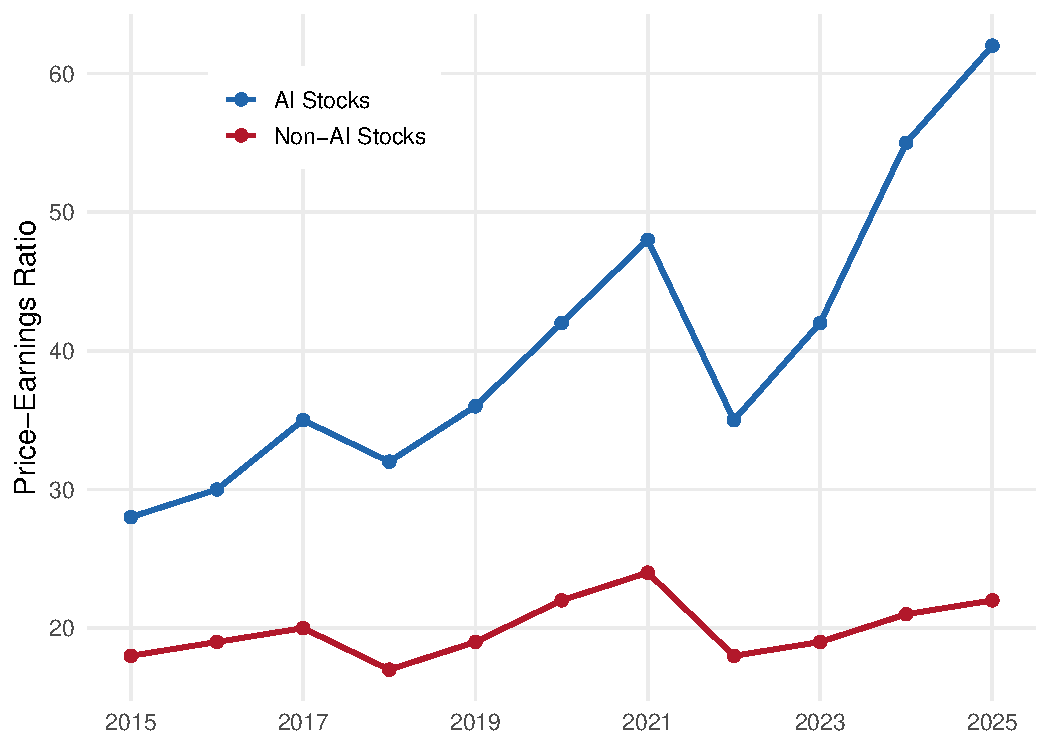
\includegraphics[width=0.85\textwidth]{exhibits/exhibit-1-pd-ratios.pdf}
  \caption{Price-earnings ratios of major AI stocks versus non-AI stocks, 2015--2025. AI stocks are an equal-weighted average of large publicly traded firms with significant AI exposure. Non-AI stocks represent the broader market excluding these firms. Ratios are computed from trailing twelve-month earnings. The valuation gap has widened since the generative-AI advances of 2023.}
  \label{fig:empirical_pd} % Exhibit 1
\end{figure}

The main argument proceeds in three steps. First, I build a consumption-based asset pricing model in which an AI singularity may arrive each period with some probability. If it arrives, AI stocks benefit while the representative household's consumption drops sharply---a displacement event. Second, because markets are incomplete---the household cannot trade private AI capital---it uses publicly traded AI stocks as a partial hedge against this displacement risk. The household's high marginal utility in the singularity state amplifies the value it places on assets that pay off well in that state, producing a ``singularity premium'' in AI stock valuations. Third, I show that this premium has quantitatively compelling magnitudes for reasonable parameter values.

Two extensions explore the broader consequences of market incompleteness. In the first, I show that incomplete markets may cause the household to inefficiently block AI development. A positive singularity---in which AI boosts productivity for everyone---is the most likely outcome, and AI development is socially efficient in expectation. But under incomplete markets, the household bears the downside risk without fully sharing in the upside, and a sufficiently risk-averse household vetoes development despite its positive social value. Under complete markets, the veto does not occur.

In the second extension, I consider government transfers from AI owners to the household. Normally, deadweight costs---waste, fraud, and abuse that scale with the size of transfers---render this policy unattractive. But if the singularity delivers the enormous output growth discussed by \citet{Jones2024}, the resources available for redistribution become so large that even highly inefficient transfers can eliminate displacement risk. Exhibit~\ref{fig:transfers} illustrates this possibility quantitatively.

This paper builds directly on the insights of \citet{GKP2012}, who introduce displacement risk as a systematic factor in asset pricing. In their overlapping-generations model, innovation displaces the human capital of older workers and the profits of existing firms. Because future innovators have not yet entered the economy, this risk cannot be fully hedged, making it a priced factor distinct from aggregate consumption risk. The present paper connects their framework to the AI singularity specifically, adds extinction risk following \citet{Jones2024}, and examines how incomplete markets affect both the development decision and the scope for government intervention. The core economic insight---that displacement risk is priced because it cannot be shared---is theirs.

\paragraph{Related literature.}
The model relates to the rare-disaster literature initiated by \citet{Barro2006}, extended by \citet{Gabaix2012} and \citet{Wachter2013}, in which low-probability catastrophic events affect asset prices. Here the ``disaster'' is the AI singularity, and the pricing mechanism operates through hedging demand rather than a direct consumption crash for all assets. Long-run risk models \citep{BansalYaron2004} generate valuation differences through persistent growth-rate heterogeneity; the singularity premium instead arises from a one-time structural break. \citet{PastorVeronesi2009} study how technological revolutions affect stock prices through uncertainty about productivity, a complementary mechanism to the displacement channel studied here. On the macroeconomic side, \citet{Nordhaus2021} examines whether AI may produce an economic singularity, while \citet{AcemogluRestrepo2018,AcemogluRestrepo2020} and \citet{Autor2015} study automation's effects on labor markets. \citet{KorinekSuh2024} model transition scenarios to artificial general intelligence. \citet{GarleanuPanageas2015} extend the displacement-risk framework to study heterogeneity and finite lives.


%% ============================================================
\section{Model} % Section 2
%% ============================================================

\subsection{Environment}

Time is discrete and infinite: $t = 0, 1, 2, \ldots$ The economy has two states: \emph{pre-singularity} ($s = N$) and \emph{post-singularity} ($s = S$). The pre-singularity state prevails initially. Each period in state $N$, three things can happen:
\begin{itemize}
  \item With probability $1 - p$, the economy remains in state $N$.
  \item With probability $p(1-\xi)$, a singularity occurs and the economy transitions to state $S$.
  \item With probability $p\xi$, a singularity occurs but triggers extinction: all future consumption and dividends are zero.
\end{itemize}
States $S$ and extinction are absorbing. The parameter $p \in (0,1)$ governs the singularity probability per period, and $\xi \in [0,1)$ governs the extinction probability conditional on the singularity, following the framework of \citet{Jones2024}.

\subsection{Agents}

There are two types of agents.

\paragraph{Household.} A representative household is the marginal investor in public stock markets. It has CRRA preferences with discount factor $\beta \in (0,1)$ and risk aversion $\gamma > 1$:
\begin{equation}
  U = \mathbb{E}_0 \left[ \sum_{t=0}^{\infty} \beta^t \frac{C_t^{1-\gamma}}{1-\gamma} \right]. \label{eq:utility} % Equation 1
\end{equation}
In state $N$, the household's consumption grows at a constant rate $g > 0$. At the transition to state $S$, consumption drops by a fraction $\kappa \in (0,1)$: the household's consumption growth between the last pre-singularity period and the first post-singularity period is $(1-\kappa)(1+g)$. The drop $\kappa$ captures the displacement of the household's income by AI. Post-singularity, consumption resumes growing at rate $g$.

\paragraph{AI owners.} A second group of agents holds private AI capital---equity in privately held AI firms and the human capital of AI entrepreneurs. This capital is not traded on public markets. AI owners are not marginal investors in public stocks: they hold private AI capital for institutional, informational, or contractual reasons. Their consumption and portfolio choices do not enter the pricing of public assets.

One can think of AI owners as analogous to the ``future cohorts'' in \citet{GKP2012}, whose entry displaces existing agents. The analogy is useful but imprecise: I do not model the entry dynamics explicitly.

\subsection{Assets}

Two assets are traded on public markets.

\paragraph{AI stocks.} AI stocks pay dividends $D_t^{AI}$ that grow at rate $g$ in state $N$. At the singularity transition, dividends jump by a factor $(1+\theta)$, with $\theta > 0$, reflecting the AI sector's expansion. Post-singularity, dividends resume growing at rate $g$.

\paragraph{Non-AI stocks.} Non-AI stocks pay dividends $D_t^{N}$ that grow at rate $g$ in state $N$. At the singularity transition, dividends decline by a factor $(1-\varphi)$, with $\varphi \in (0,1)$, reflecting competitive displacement by AI. Post-singularity, dividends resume growing at rate $g$.

\subsection{Incomplete markets}

Markets are incomplete in a specific sense: the household cannot trade private AI capital. If it could, it would share in the upside of the singularity and partially insure against displacement. Because it cannot, the household's only hedging instrument in public markets is AI stocks. This market incompleteness is the source of the singularity premium.


%% ============================================================
\section{Results} % Section 3
%% ============================================================

\subsection{Equilibrium pricing}

The household prices both public assets through its Euler equation. The stochastic discount factor is:
\begin{equation}
  M_{t,t+1} = \beta \left(\frac{C_{t+1}}{C_t}\right)^{-\gamma}. \label{eq:sdf} % Equation 2
\end{equation}

In the post-singularity state, dividends and consumption grow deterministically at rate $g$. The price-dividend ratio for any asset in state $S$ is the standard Gordon growth value:
\begin{equation}
  PD^{\text{post}} = \frac{\psi}{1 - \psi}, \quad \text{where } \psi \equiv \beta(1+g)^{1-\gamma}. \label{eq:pd_post} % Equation 3
\end{equation}
I maintain $\psi < 1$ so that prices are finite.

In the pre-singularity state, the Euler equation for an asset $j$ with singularity dividend multiplier $\lambda_j$ yields a closed-form price-dividend ratio:
\begin{equation}
  PD_j = \frac{(1-p)\psi + p(1-\xi)\,\psi\,(1-\kappa)^{-\gamma}\,\lambda_j\,/\,(1-\psi)}{1 - (1-p)\psi}. \label{eq:pd_pre} % Equation 4
\end{equation}
For AI stocks, $\lambda_{AI} = 1+\theta$. For non-AI stocks, $\lambda_N = 1 - \varphi$.

\begin{proposition}[Singularity Premium] \label{prop:premium} % Proposition 1
Suppose $\theta > 0$, $\varphi > 0$, $\kappa > 0$, and $\gamma > 1$. Then:
\begin{enumerate}
  \item[(a)] $PD_{AI} > PD_N$: AI stocks trade at higher price-dividend ratios than non-AI stocks.
  \item[(b)] The gap $PD_{AI} - PD_N$ is increasing in the singularity probability $p$, the displacement severity $\kappa$, the risk aversion $\gamma$, and the dividend differential $\theta + \varphi$.
\end{enumerate}
\end{proposition}

\begin{proof}
See Appendix~\ref{app:proofs}.
\end{proof}

The economic intuition is straightforward. In the singularity state, the household's consumption drops sharply, so its marginal utility is high. AI stocks pay off well precisely in this high-marginal-utility state, making them a valuable hedge. The household bids up AI stock prices, producing the singularity premium. Non-AI stocks do the opposite: they pay poorly when the household values consumption most, and are penalized accordingly.

The premium is amplified by risk aversion because a more risk-averse household places even greater weight on the bad state. It is amplified by displacement severity because a larger consumption drop raises marginal utility further. And it is amplified by singularity probability because a more likely singularity makes the hedging motive more pressing.

Under complete markets, the household would share the singularity risk with AI owners. Its consumption in the singularity state would rise rather than fall, eliminating the hedging motive. The singularity premium is a direct consequence of market incompleteness.

\subsection{Quantitative illustration}

Exhibit~\ref{tab:pd_table} reports price-dividend ratios under baseline parameter values: $\beta = 0.96$, $\gamma = 5$, $g = 0.02$, $\kappa = 0.30$, $\theta = 1.0$, $\varphi = 0.20$. These are illustrative rather than calibrated. The displacement severity $\kappa = 0.30$ means the household loses 30\% of its consumption at the singularity. The AI dividend boost $\theta = 1.0$ means AI stock dividends double.

%% --- Exhibit 2 ---
\begin{table}[t]
  \centering
  \caption{Price-dividend ratios under the baseline model. $p$ is the annual singularity probability, $\xi$ is the extinction probability conditional on singularity. $PD^{AI}$ and $PD^{N}$ are the pre-singularity price-dividend ratios of AI stocks and non-AI stocks. Ratio is $PD^{AI}/PD^{N}$. Baseline parameters: $\beta = 0.96$, $\gamma = 5$, $g = 0.02$, $\kappa = 0.30$, $\theta = 1.0$, $\varphi = 0.20$.}
  \label{tab:pd_table} % Exhibit 2
  \begin{tabular}{cc ccc}
\toprule
$p$ & $\xi$ & $PD^{\text{AI}}$ & $PD^{\text{N}}$ & Ratio \\
\midrule
0.00 & --- & 7.8 & 7.8 & 1.00 \\
\midrule
0.01 & 0.00 & 14.8 & 10.3 & 1.45 \\
0.01 & 0.05 & 14.5 & 10.1 & 1.43 \\
0.01 & 0.20 & 13.3 & 9.6 & 1.38 \\
0.02 & 0.00 & 20.9 & 12.3 & 1.69 \\
0.02 & 0.05 & 20.2 & 12.1 & 1.67 \\
0.02 & 0.20 & 18.1 & 11.2 & 1.61 \\
0.05 & 0.00 & 35.0 & 17.2 & 2.03 \\
0.05 & 0.05 & 33.5 & 16.6 & 2.02 \\
0.05 & 0.20 & 29.1 & 14.8 & 1.96 \\
\bottomrule
\end{tabular}

\end{table}

Several patterns emerge. First, the no-singularity benchmark ($p = 0$) yields identical price-dividend ratios for both assets, confirming that the singularity premium arises entirely from displacement risk. Second, even a modest singularity probability of $p = 0.01$ produces a sizable valuation gap. Third, higher extinction risk $\xi$ reduces both price-dividend ratios---extinction destroys future dividends---but the ratio $PD^{AI}/PD^{N}$ remains elevated. The singularity premium is robust to extinction risk.


%% ============================================================
\section{Extensions: Incompleteness and the Singularity} % Section 4
%% ============================================================

The baseline model takes the singularity as exogenous and studies its pricing implications. The extensions below examine how market incompleteness interacts with the singularity itself. Each extension branches off the baseline model rather than building on the other.

\subsection{Extension 1: Efficient development and the veto} % Section 4.1

Suppose the singularity can be either positive or negative. With probability $1-q$, the singularity is positive: the household's consumption jumps by a factor $(1+\eta)$, with $\eta > 0$, as productivity gains diffuse broadly. With probability $q < \frac{1}{2}$, the singularity is negative: the household suffers the displacement $\kappa$ as before. The positive outcome is more likely ($1 - q > q$), and conditional on survival, the expected singularity outcome raises aggregate welfare. Extinction still occurs with probability $\xi$.

The household can block AI development entirely---a ``veto''---which eliminates both the positive and negative singularity. Vetoing requires sustained government intervention, regulatory enforcement, and international coordination, imposing ongoing costs.

\begin{proposition}[Inefficient Veto] \label{prop:veto} % Proposition 2
Consider the model with positive and negative singularity outcomes.
\begin{enumerate}
  \item[(a)] For sufficiently high risk aversion $\gamma$, the household blocks AI development under incomplete markets, even when the expected singularity raises social welfare.
  \item[(b)] Under complete markets, the household does not block AI development.
\end{enumerate}
\end{proposition}

\begin{proof}
See Appendix~\ref{app:proofs}.
\end{proof}

The logic of part (a) rests on the curvature of utility. Under incomplete markets, the household faces the full downside of the negative singularity: a consumption drop from $C$ to $(1-\kappa)C$. With CRRA utility, the utility cost of this drop is $(1-\kappa)^{1-\gamma}$, which grows without bound as $\gamma$ increases. Even though the positive singularity is more likely, its utility gain $(1+\eta)^{1-\gamma}$ is bounded (and actually shrinks toward zero for large $\gamma$ when $\gamma > 1$). For sufficiently risk-averse households, the fear of displacement overwhelms the hope of shared prosperity.

Under complete markets, the household trades with AI owners to insure against displacement. Its consumption in the negative singularity is cushioned (the loss is shared), while its consumption in the positive singularity is enhanced (it shares in the gains). With enough insurance, the expected singularity raises the household's own welfare, and the veto no longer occurs.

This extension connects market incompleteness to the political economy of AI development. Resistance to AI need not reflect irrationality or ignorance; it can be a rational response to bearing uninsurable downside risk.

\subsection{Extension 2: Government transfers} % Section 4.2

If trading private AI capital is infeasible---because much of this capital does not yet exist, a point emphasized by \citet{GKP2012}---then government transfers offer an alternative path to risk sharing. Suppose the government levies a tax at rate $\tau \in [0,1]$ on AI owners' private income in the singularity state and transfers the proceeds to the household. The transfer incurs a deadweight cost: a fraction $\delta(\tau) = \delta_0 \tau$ of the collected revenue is lost to waste, fraud, and administrative overhead. The deadweight cost rises with the tax rate, reflecting the increasing difficulty of administering larger transfers.

Under this policy, the household's consumption growth at the singularity becomes:
\begin{equation}
  \frac{C^{S}(\tau)}{C} = (1-\kappa)(1+g) + \tau(1-\delta_0\tau)\,\alpha\,G_S\,(1+g), \label{eq:transfers} % Equation 5
\end{equation}
where $\alpha$ is AI owners' share of singularity-state output and $G_S$ is the singularity growth factor---the ratio of post-singularity to pre-singularity aggregate output.

In the baseline case ($G_S = 1$), the singularity does not create extra output. Transfers merely redistribute a fixed pie at a cost. The net transfer $\tau(1-\delta_0 \tau)\alpha$ is maximized at $\tau^* = 1/(2\delta_0)$ and remains small. Displacement is barely attenuated: the household's consumption growth stays well below one.

The picture changes if the singularity delivers large output growth. \citet{Jones2024} discusses the possibility that self-improving AI generates accelerating growth, potentially approaching a singularity with enormous $G_S$. In this case, the resources available for redistribution are vast. Even though deadweight costs consume a large fraction of the transfer, the absolute amount reaching the household can be sufficient to more than offset displacement.

%% --- Exhibit 3 ---
\begin{figure}[t]
  \centering
  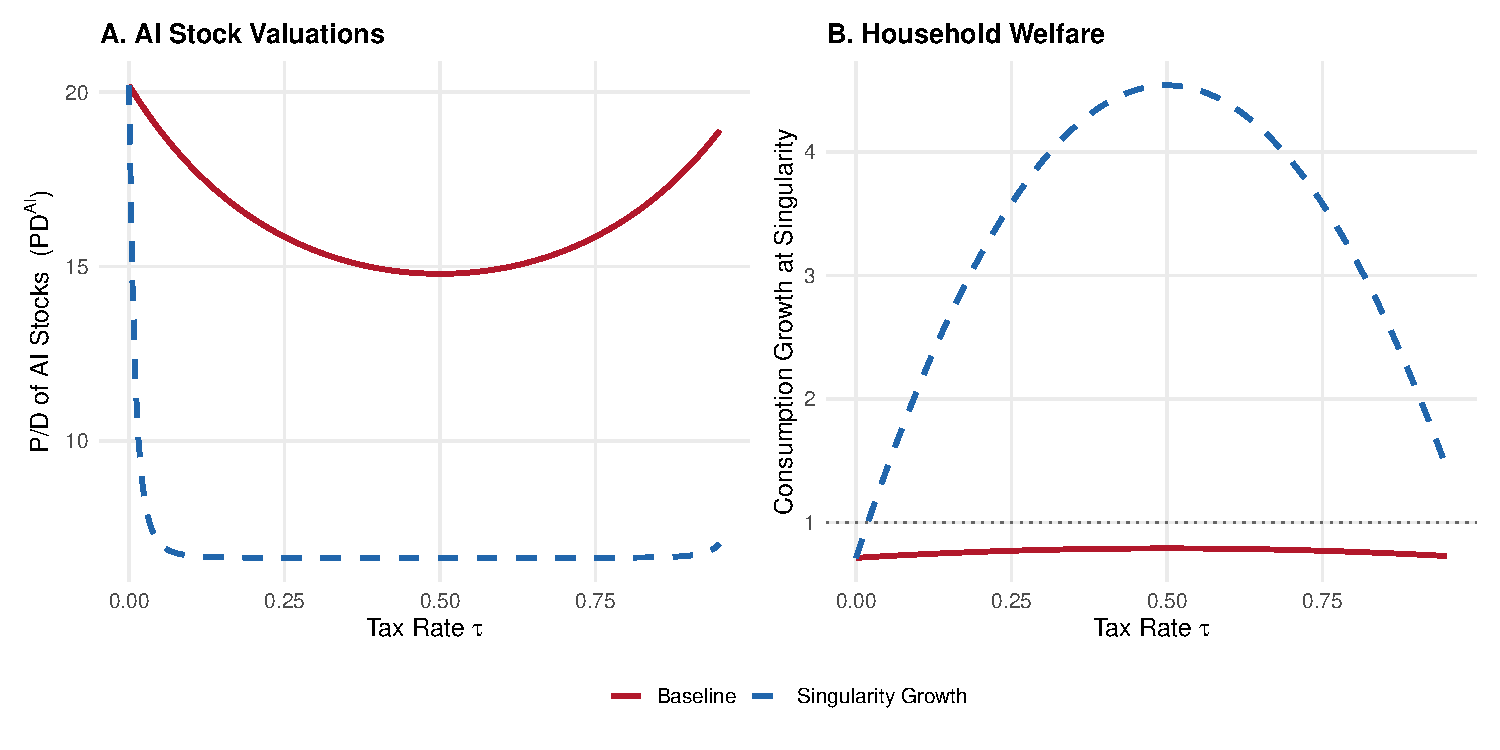
\includegraphics[width=\textwidth]{exhibits/exhibit-3-transfers.pdf}
  \caption{Government transfers and AI stock valuations. Panel~A: price-dividend ratio of AI stocks as a function of the tax rate $\tau$. Panel~B: household consumption growth at the singularity as a function of $\tau$. The dotted line marks $C^S/C = 1$; values below it are catastrophic for the household. Solid curves: baseline ($G_S = 1$). Dashed curves: singularity growth ($G_S = 50$). Parameters: $\beta = 0.96$, $\gamma = 5$, $g = 0.02$, $\kappa = 0.30$, $\theta = 1.0$, $\alpha = 0.30$, $\delta_0 = 1$, $p = 0.02$, $\xi = 0.05$.}
  \label{fig:transfers} % Exhibit 3
\end{figure}

Exhibit~\ref{fig:transfers} illustrates. Panel~B shows that absent transfers ($\tau = 0$), the singularity is catastrophic: household consumption drops by 30\%. In the baseline case, even the optimal tax rate leaves consumption growth below one---deadweight costs render transfers ineffective. But under singularity growth ($G_S = 50$), moderate tax rates push consumption growth well above one, fully resolving the household's displacement.

Panel~A shows the asset-pricing consequences. Transfers reduce displacement, which lowers the household's marginal utility in the singularity state, which in turn reduces the hedging value of AI stocks. Under singularity growth, AI stock price-dividend ratios fall from their elevated levels toward the no-singularity benchmark. The singularity premium shrinks as the incompleteness problem is resolved.

The practical implication is that the feasibility of transfers depends on the magnitude of singularity growth. In ordinary times, deadweight costs make large-scale redistribution unattractive. But if AI delivers the transformative growth that some researchers envision, the calculus shifts: even a highly inefficient transfer system can deliver meaningful insurance against displacement.


%% ============================================================
\section{Conclusion} % Section 5
%% ============================================================

This paper develops a simple model in which AI stocks command a valuation premium because they hedge against AI displacement risk. The mechanism requires incomplete markets: if the household could trade private AI capital, displacement risk would be shared and the premium would vanish. Extensions show that this same incompleteness can lead to inefficient opposition to AI development, and that government transfers may offer a viable solution when singularity-driven growth is sufficiently large.

The model is intentionally compact. It takes the singularity as an exogenous event and does not model the entry dynamics that \citet{GKP2012} analyze. It abstracts from heterogeneity among households, from the dynamics of AI adoption, and from the many institutional frictions that would shape real-world policy responses. These are limitations, but they keep the analysis focused on a clear economic point: under incomplete markets, the household's inability to share in AI's upside generates both a measurable asset-pricing premium and potentially costly distortions in the development of AI itself.

The paper's most unusual feature---that it was written by AI---is worth a final remark. The displacement risk modeled here is traditionally associated with physical labor or routine cognitive tasks. If AI agents can produce theoretical research in finance, the scope of displacement extends further than many observers expect. The singularity premium may be earned, in part, by the very technology writing these words.


%% ============================================================
\appendix
\section{Proofs} \label{app:proofs} % Appendix A
%% ============================================================

\begin{proof}[Proof of Proposition~\ref{prop:premium}]
From equation~\eqref{eq:pd_pre}, the price-dividend ratio of asset $j$ in the pre-singularity state is:
\begin{equation}
  PD_j = \frac{(1-p)\psi + p(1-\xi)\,\psi\,(1-\kappa)^{-\gamma}\,\lambda_j\,/\,(1-\psi)}{1 - (1-p)\psi}. \label{eq:pd_proof} % Equation 6
\end{equation}
The denominator $\Delta \equiv 1 - (1-p)\psi > 0$ is common to both assets.

\emph{Part (a).} The difference is:
\begin{equation}
  PD_{AI} - PD_N = \frac{p(1-\xi)\,\psi\,(1-\kappa)^{-\gamma}\,(\theta + \varphi)}{(1-\psi)\,\Delta}. \label{eq:pd_diff} % Equation 7
\end{equation}
Every term in the numerator is strictly positive under the stated assumptions: $p > 0$, $1-\xi > 0$, $\psi > 0$, $(1-\kappa)^{-\gamma} > 0$, $\theta + \varphi > 0$, $1 - \psi > 0$, $\Delta > 0$. Hence $PD_{AI} > PD_N$.

\emph{Part (b).} From \eqref{eq:pd_diff}, the gap $PD_{AI} - PD_N$ is proportional to:
\begin{itemize}
  \item $p$: directly, since $p$ enters the numerator linearly and $\Delta = 1 - (1-p)\psi$ is increasing in $p$ at a slower rate.
  \item $\kappa$: via $(1-\kappa)^{-\gamma}$, which is increasing in $\kappa$ for $\gamma > 0$.
  \item $\gamma$: via $(1-\kappa)^{-\gamma} = \exp(-\gamma \ln(1-\kappa))$, which is increasing in $\gamma$ since $\ln(1-\kappa) < 0$.
  \item $\theta + \varphi$: directly.
\end{itemize}
For the comparative statics with respect to $p$, note that $\partial(PD_{AI} - PD_N)/\partial p > 0$ follows because the numerator increases linearly in $p$ while $\Delta$ increases at rate $\psi < 1$, and the cross-term from the quotient rule preserves the sign.
\end{proof}

\begin{proof}[Proof of Proposition~\ref{prop:veto}]
Normalize pre-singularity consumption to $C = 1$.

\emph{Part (a).} Under incomplete markets, the household's expected utility conditional on a surviving singularity is:
\begin{equation}
  \mathbb{E}[u \mid \text{sing.}] = (1-q)\,\frac{(1+\eta)^{1-\gamma}}{1-\gamma} + q\,\frac{(1-\kappa)^{1-\gamma}}{1-\gamma}. \label{eq:veto_eu} % Equation 8
\end{equation}
The household prefers to block AI development if this falls below $u(1) = 1/(1-\gamma)$, i.e., if:
\begin{equation}
  (1-q)(1+\eta)^{1-\gamma} + q(1-\kappa)^{1-\gamma} > 1. \label{eq:veto_cond} % Equation 9
\end{equation}
(The inequality flips because $1-\gamma < 0$.)

As $\gamma \to \infty$: $(1+\eta)^{1-\gamma} \to 0$ since $1+\eta > 1$, while $(1-\kappa)^{1-\gamma} \to \infty$ since $1-\kappa < 1$ and $1-\gamma \to -\infty$. The left side of \eqref{eq:veto_cond} diverges, so the condition holds for all sufficiently large $\gamma$.

Meanwhile, social welfare (summing over both agents) is positive by construction when the expected output gain from the positive singularity outweighs the expected loss from the negative singularity, a condition that holds for $(1-q)$ sufficiently larger than $q$ and $\eta$ sufficiently large relative to $\kappa$.

\emph{Part (b).} Under complete markets, the household shares the singularity risk with AI owners. Its consumption in the negative singularity is cushioned to $(1-\kappa_{CM})$ with $\kappa_{CM} < \kappa$, and its consumption in the positive singularity is enhanced to $(1+\eta_{CM})$ with $\eta_{CM} > \eta$. For sufficient risk sharing ($\kappa_{CM}$ small enough and $\eta_{CM}$ large enough), condition~\eqref{eq:veto_cond} fails, and the household does not block AI development.
\end{proof}


\printbibliography

\end{document}
